
\chapter{洞察}
\label{chap:insight}

\begin{example}[消失的方块]证明:$31.5=32.5$。

  \centering
  \begin{tikzpicture}[scale=0.6,line join=round]
    \begin{scope}[shift={(0,0)}]
      \draw[very thick,pattern=north east lines, pattern color=black](1,1)--(9,1)--(9,4)--cycle;
      \draw[very thick,pattern=dots, pattern color=red](9,1)--(14,1)--(14,3)--(11,3)--(11,2)--(9,2)--cycle;
      \draw[very thick,pattern=bricks, pattern color=blue](14,3)--(11,3)--(11,2)--(9,2)--(9,4)--(14,4)--cycle;
      \draw[very thick,pattern=checkerboard, pattern color=violet](9,4)--(14,4)--(14,6)--cycle;
      % \draw[very thick](1,1)--(14,1)--(14,6)--(9,4)--cycle;
      \draw[help lines](0,0)grid(15,7);
    \end{scope}
    \begin{scope}[shift={(0,-8)}]
      \draw[very thick,xshift=5cm,yshift=2cm,pattern=north east lines, pattern color=black](1,1)--(9,1)--(9,4)--cycle;
      \draw[very thick,pattern=dots, pattern color=red](9,1)--(14,1)--(14,3)--(11,3)--(11,2)--(9,2)--cycle;
      \draw[very thick,xshift=-3cm,yshift=-1cm,pattern=bricks, pattern color=blue](14,3)--(11,3)--(11,2)--(9,2)--(9,4)--(14,4)--cycle;
      \draw[very thick,xshift=-8cm,yshift=-3cm,pattern=checkerboard, pattern color=violet](9,4)--(14,4)--(14,6)--cycle;
      \draw[help lines](0,0)grid(15,7);
      % \draw[very thick](1,1)--(14,1)--(14,6)--(6,3)--cycle;
    \end{scope}
  \end{tikzpicture}
\end{example}

\begin{proof}
  考虑阴影部分总面积,由上图,其面积为$\dfrac12\times13\times5=32.5$;由下图,其面积为$32.5-1=31.5$。而上下两图都是由相同组件组成,其面积应相同,从而有$32.5=31.5$。
\end{proof}

请指出上述证明中的错误之处。\hints 最大的“三角形”并不是真正的三角形。


\begin{example}数一数,下面的图中有多少个三角形?
  \begin{center}
    \begin{tikzpicture}[scale=1.0]
      \coordinate(A) at (0,0);
      \coordinate(B) at (1,0);
      \coordinate(C) at (2,0);
      \coordinate(D) at (3,0);
      \coordinate(F) at (1.5,2);
      \coordinate(E) at ($.5*(D)+.5*(F)$);
      \coordinate(G) at ($.75*(B)+.25*(F)$);
      \coordinate(H) at ($.6*(C)+.4*(F)$);
      \draw(A)--(D)--(F)--(A)--(G)--(H)--(E) (B)--(F)--(C);
    \end{tikzpicture}
  \end{center}
\end{example}

\begin{example}数一数,下面的图形中有多少个四边形?
  \begin{center}
    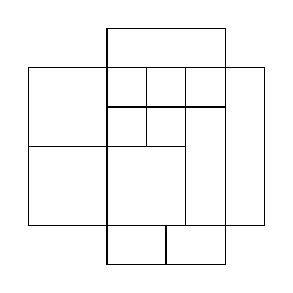
\begin{tikzpicture}[scale=.5]
      \draw(0,1)rectangle(6,5);
      \draw(2,0)rectangle(5,6);
      \draw(0,3)--(4,3)
           (3.5,0)--(3.5,1)
           (4,1)--(4,5)
           (2,4)--(5,4)
           (3,3)--(3,5);
    \end{tikzpicture}
  \end{center}
\end{example}
\begin{proof}[提示]首先最小的由单个四边形组成的共有13个。
  \begin{center}
    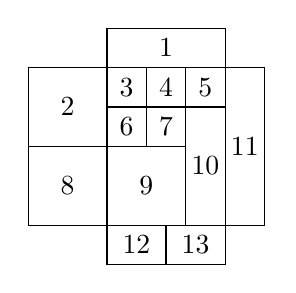
\begin{tikzpicture}[scale=.5]
      \draw(0,1)rectangle(6,5);
      \draw(2,0)rectangle(5,6);
      \draw(0,3)--(4,3)
           (3.5,0)--(3.5,1)
           (4,1)--(4,5)
           (2,4)--(5,4)
           (3,3)--(3,5);
           \foreach \n/\x/\y in{%
             1/3.5/5.5, 2/1/4, 3/2.5/4.5, 4/3.5/4.5, 5/4.5/4.5, 6/2.5/3.5, 7/3.5/3.5,
             8/1/2, 9/3/2, 10/4.5/2.5, 11/5.5/3, 12/2.75/.5, 13/4.25/.5}{%
             \node at(\x,\y){\n};
           }
    \end{tikzpicture}
  \end{center}

  由两个小四边形组成的共有9个:
  \begin{center}
    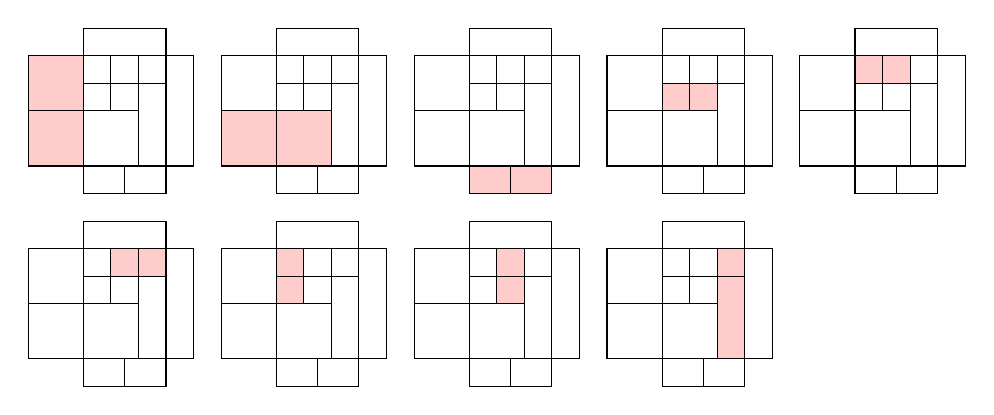
\begin{tikzpicture}[scale=.35]
      \foreach \dx/\dy/\x/\y/\xx/\yy in {%
        0/0/0/1/2/5, 7/0/0/1/4/3, 14/0/2/0/5/1, 21/0/2/3/4/4, 28/0/2/4/4/5, 
        0/7/3/4/5/5, 7/7/2/3/3/5, 14/7/3/3/4/5, 21/7/4/1/5/5
      }{
        \begin{scope}[shift={(\dx,-\dy)}]
          \fill[color=red!20](\x,\y)rectangle(\xx,\yy);
          \draw(0,1)rectangle(6,5);
          \draw(2,0)rectangle(5,6);
          \draw(0,3)--(4,3) (3.5,0)--(3.5,1) (4,1)--(4,5) (2,4)--(5,4) (3,3)--(3,5);
        \end{scope}
      }
    \end{tikzpicture}    
  \end{center}

  由三个小四边形组成的共有4个:
  \begin{center}
    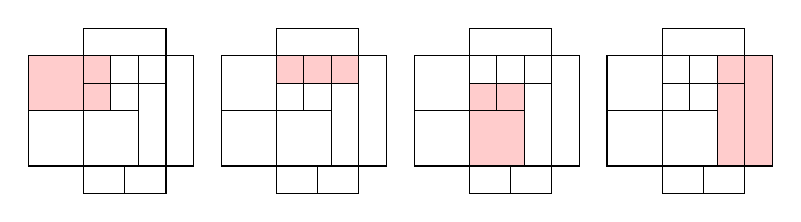
\begin{tikzpicture}[scale=.35]
      \foreach \dx/\dy/\x/\y/\xx/\yy in {%
        0/0/0/3/3/5, 7/0/2/4/5/5, 14/0/2/1/4/4, 21/0/4/1/6/5
      }{
        \begin{scope}[shift={(\dx,-\dy)}]
          \fill[color=red!20](\x,\y)rectangle(\xx,\yy);
          \draw(0,1)rectangle(6,5);
          \draw(2,0)rectangle(5,6);
          \draw(0,3)--(4,3) (3.5,0)--(3.5,1) (4,1)--(4,5) (2,4)--(5,4) (3,3)--(3,5);
        \end{scope}
      }
    \end{tikzpicture}    
  \end{center}
  
  由四个小四边形组成的共有3个:
  \begin{center}
    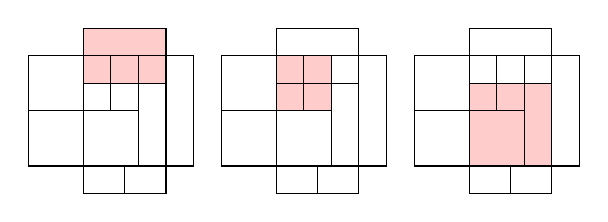
\begin{tikzpicture}[scale=.35]
      \foreach \dx/\dy/\x/\y/\xx/\yy in {%
        0/0/2/4/5/6, 7/0/2/3/4/5, 14/0/2/1/5/4
      }{
        \begin{scope}[shift={(\dx,-\dy)}]
          \fill[color=red!20](\x,\y)rectangle(\xx,\yy);
          \draw(0,1)rectangle(6,5);
          \draw(2,0)rectangle(5,6);
          \draw(0,3)--(4,3) (3.5,0)--(3.5,1) (4,1)--(4,5) (2,4)--(5,4) (3,3)--(3,5);
        \end{scope}
      }
    \end{tikzpicture}    
  \end{center}

  其余的自行考虑。
\end{proof}